\documentclass[border=10pt]{standalone}

\usepackage{tikz}
\usepackage{tikzsymbols}
\usetikzlibrary{calc,patterns,shapes.geometric}

\def\centerarc[#1](#2)(#3:#4:#5){\draw[#1] ($(#2)+({#5*cos(#3)},{#5*sin(#3)})$) arc (#3:#4:#5);}

\begin{document}
	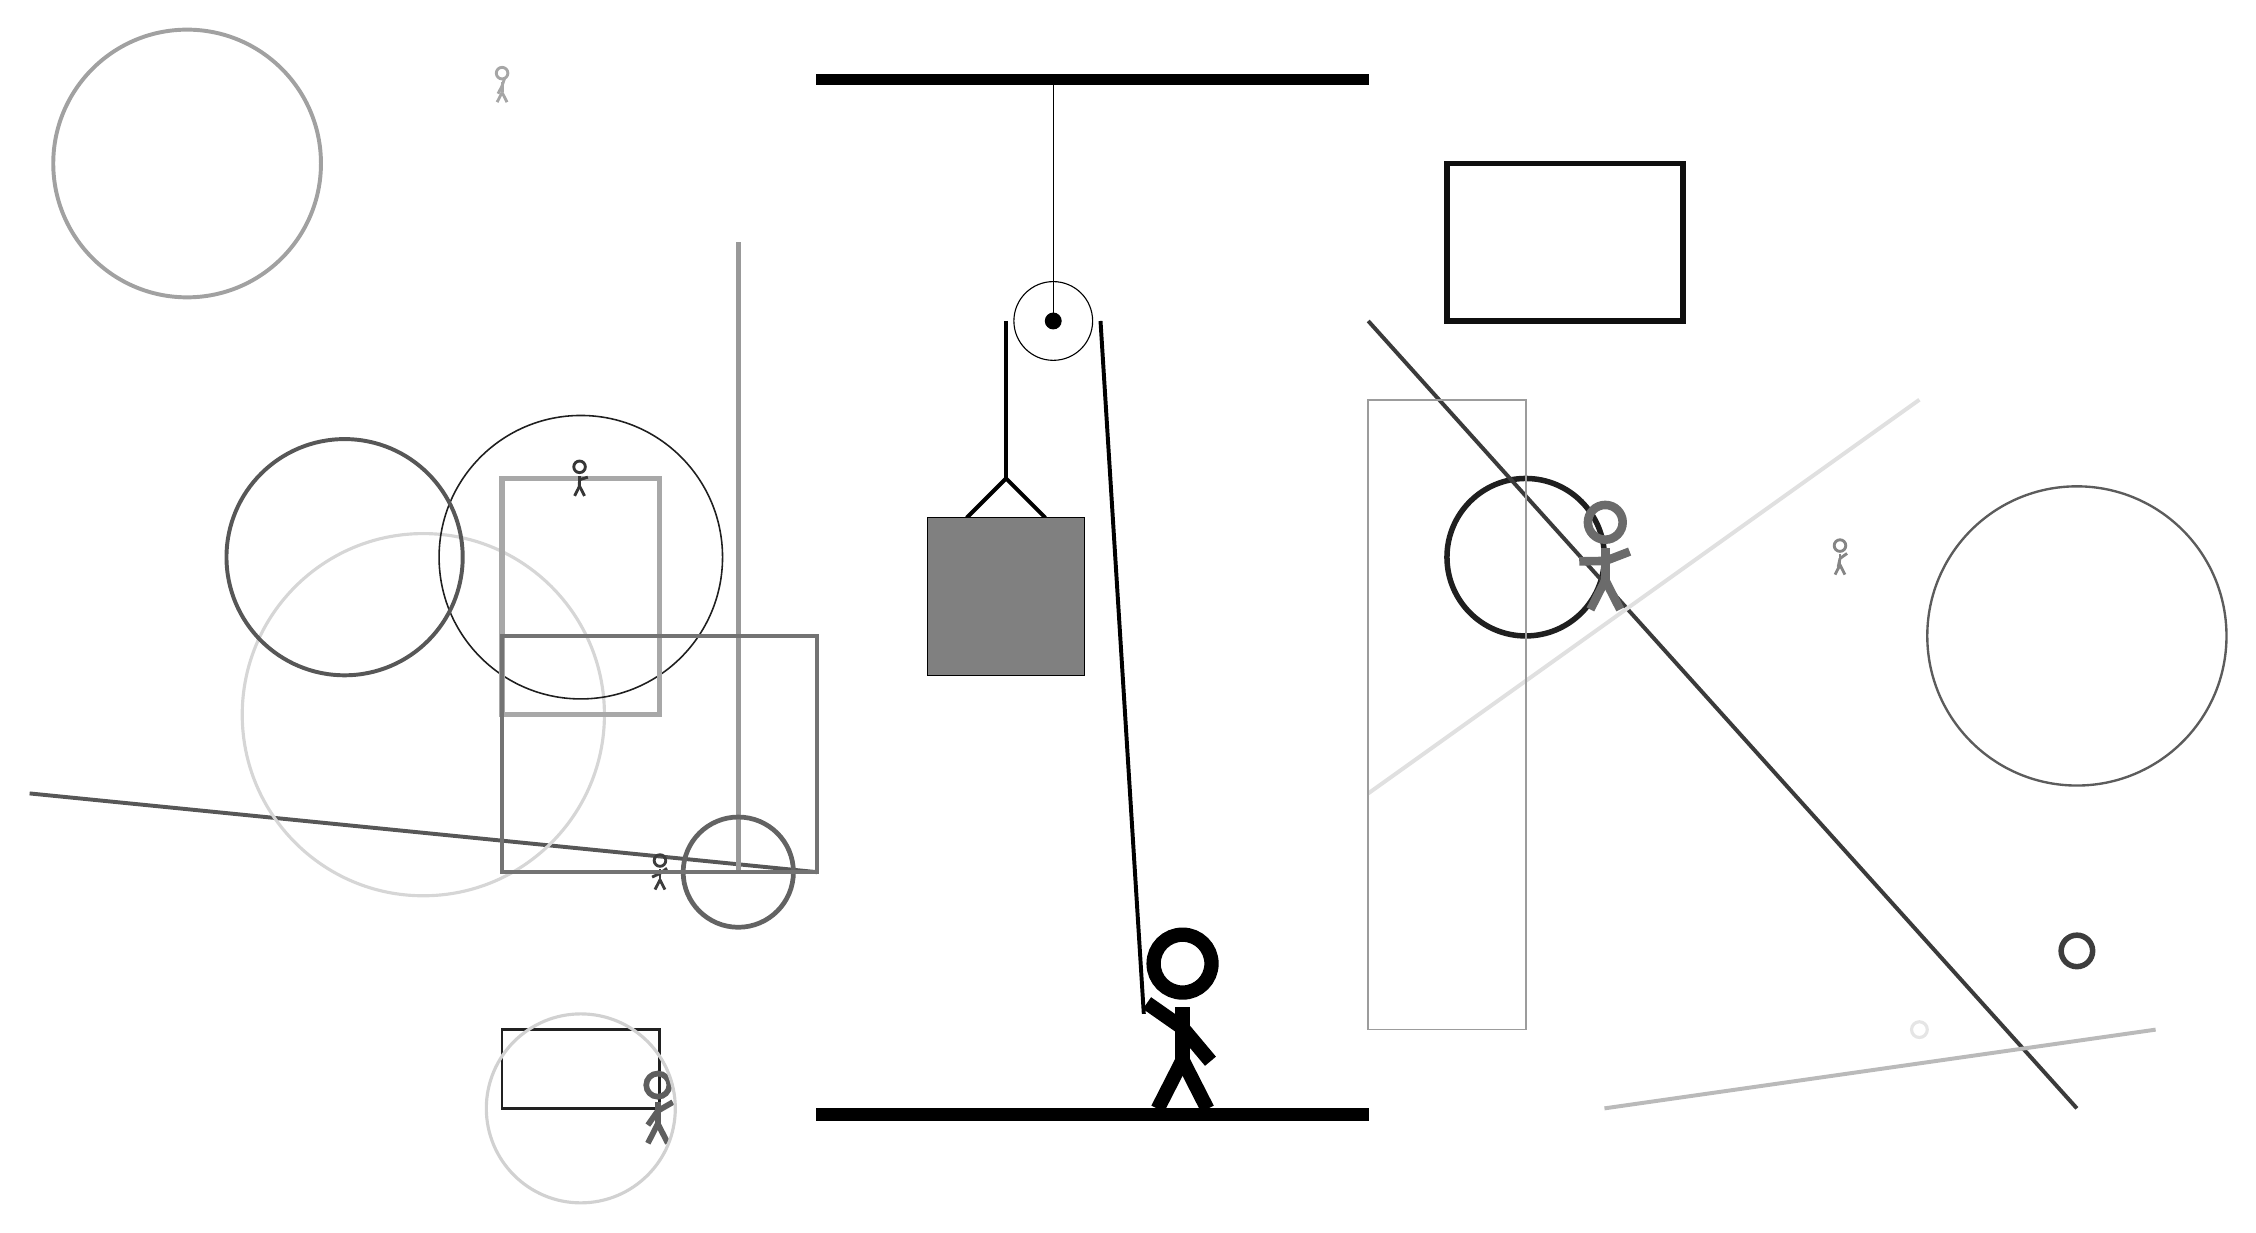
\begin{tikzpicture}
		%%%%% START %%%%%
		
		\draw[fill=black] (-2, 10) rectangle (5, 10.125);
		
		\draw (1, 7) circle (0.5);
		\draw[fill=black] (1, 7) circle (0.1);
		\draw (1, 10) -- (1, 7);
		
		\draw[line width=0.5mm] (-0.1, 4.5) -- (0.4, 5.0) -- (0.9, 4.5);
		\draw[fill=black!50] (-0.6, 4.5) rectangle (1.4, 2.5);
		
		\draw[line width=0.5mm, color=black!66](-2, 0) -- (-12, 1);
		
		\draw [line width=0.7mm, color=black!88](7, 4) circle (1.0);
		\draw[line width=0.5mm, color=black!77](5, 7) -- (14, -3);
		\node[line width=0.5mm, color=black!35] at (-6, 10) {\Strichmaxerl[2][62][72]};
		\draw[line width=0.7mm, color=black!40] (-3, 0) rectangle (-3, 8);
		
		\draw [line width=0.5mm, color=black!37](-10, 9) circle (1.7);
		\node[line width=0.3mm, color=black!48] at (11, 4) {\Strichmaxerl[2][78][35]};
		\draw[line width=0.3mm, color=black!87] (-4, -2) rectangle (-6, -3);
		\draw[line width=0.7mm, color=black!94] (6, 9) rectangle (9, 7);
		\node[line width=0.6mm, color=black!76] at (-4, 0) {\Strichmaxerl[2][25][36]};
		\draw [line width=0.7mm, color=black!76](14, -1) circle (0.2);
		\draw [line width=0.4mm, color=black!16](-7, 2) circle (2.3);
		\draw [line width=0.2mm, color=black!88](-5, 4) circle (1.8);
		\node[line width=0.5mm, color=black!63] at (-4, -3) {\Strichmaxerl[4][55][30]};
		\draw[line width=0.5mm, color=black!12](5, 1) -- (12, 6);
		\draw [line width=0.6mm, color=black!61](-3, 0) circle (0.7);
		\draw [line width=0.5mm, color=black!66](-8, 4) circle (1.5);
		
		\draw [line width=0.4mm, color=black!18](-5, -3) circle (1.2);
		\draw [line width=0.3mm, color=black!64](14, 3) circle (1.9);
		\draw [line width=0.4mm, color=black!10](12, -2) circle (0.1);
		\draw[line width=0.5mm, color=black!27](8, -3) -- (15, -2);
		
		\node[line width=0.7mm, color=black!58] at (8, 4) {\Strichmaxerl[6][1][21]};
		
		\draw[line width=0.7mm, color=black!34] (-4, 2) rectangle (-6, 5);
		\draw[line width=0.2mm, color=black!39] (5, 6) rectangle (7, -2);
		\draw[line width=0.5mm, color=black!55] (-2, 0) rectangle (-6, 3);
		
		\node[line width=0.4mm, color=black!79] at (-5, 5) {\Strichmaxerl[2][87][17]};
		
		\draw[line width=0.5mm] (0.4, 7) -- (0.4, 5.0);
		\centerarc[line width=0.5mm](1, 7)(0:180:0.6);
		\draw[line width=0.5mm](1.6, 7) -- (2.15, -1.8);
		
		\node at (2.6, -1.9) {\Strichmaxerl[10][-35][-50]};
		
		\draw[fill=black] (-2, -3) rectangle (5, -3.15);
		
		%%%%% END %%%%%
	\end{tikzpicture}
\end{document}